\chapter{Future Work}
1. ViT might work better with pre-processing e.g. cropping + yuv TBD

% Maybe entropy and other distance metrics, one day

%%%%%%%%%%%%%%%%%%%%%%%
% ENTROPY RESULTS RAW %
%%%%%%%%%%%%%%%%%%%%%%%

% We'll select one case - e.g. 5 bins balanced 
% and put the rest in appendix
% Fonts need tweaking as some are cut/bleeding

% 15_BINS_CNN_SOFTMAX_DIST_BALANCED

% \subsection{Average Entropy Prediction of cnn model trained on 15 bin balanced Dataset}

% \begin{figure}[H]
%     \centering
%     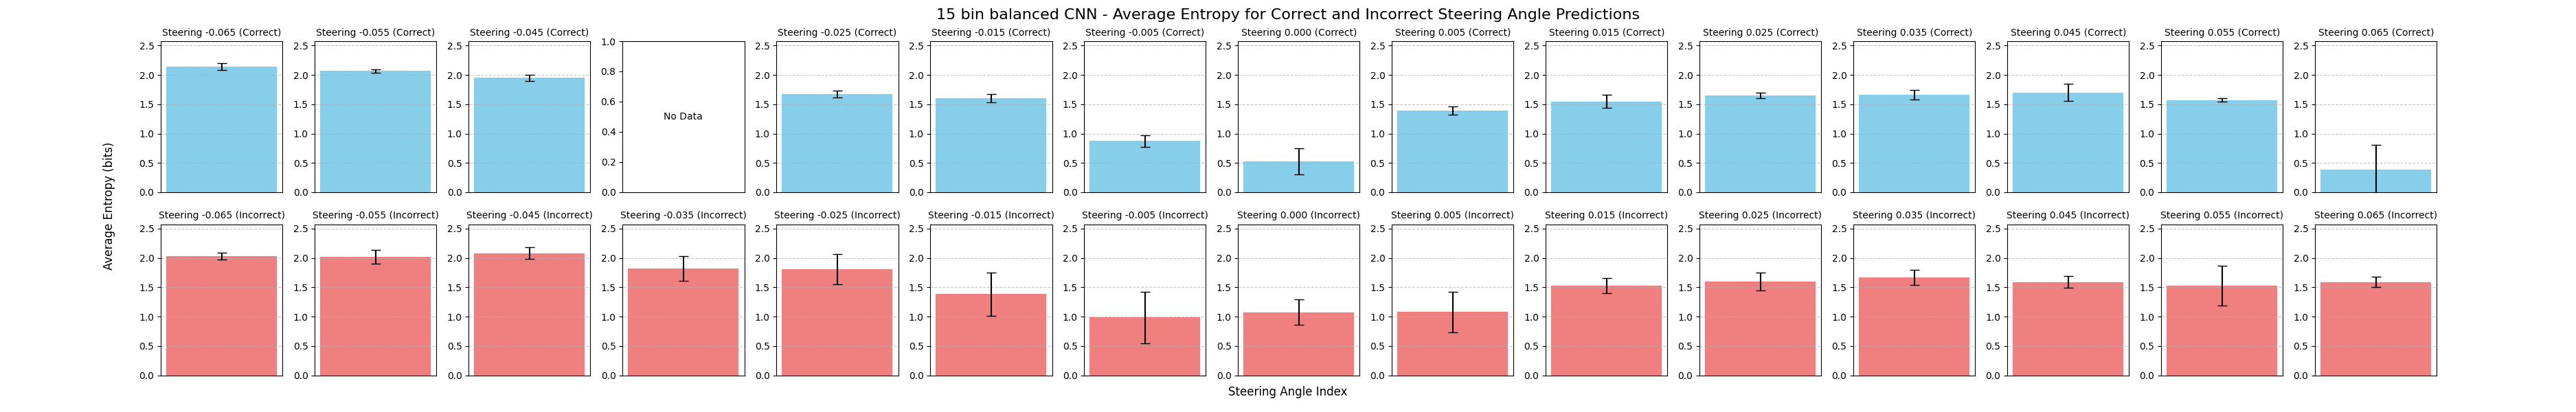
\includegraphics[width=1\linewidth]{Figures/Results/15_bins_cnn_entropy_plot_balanced.png}
%     \caption{Average Entropy for Correct and Incorrect Steering Angles Predictions for the 15-Bin cnn Model on a balanced Dataset, with Error Bars Indicating Standard Deviation.}
%     \label{fig:15_bins_cnn_entropy_balanced}
% \end{figure}
% % 15_BINS_CNN_SOFTMAX_DIST_UNBALANCED

% \subsection{Average Entropy Prediction of cnn model trained on 15 bin unbalanced Dataset}

% \begin{figure}[H]
%     \centering
%     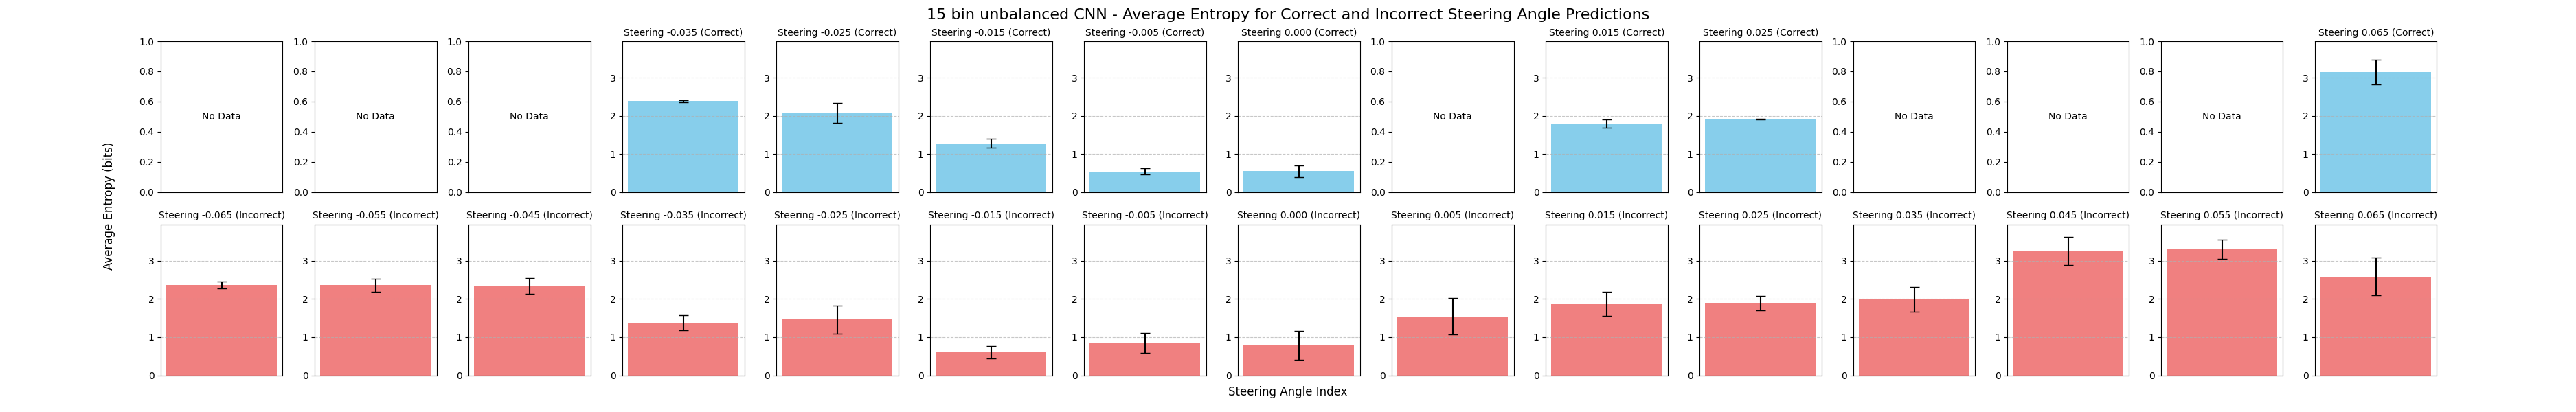
\includegraphics[width=1\linewidth]{Figures/Results/15_bins_cnn_entropy_plot_unbalanced.png}
%     \caption{Average Entropy for Correct and Incorrect Steering Angles Predictions for the 15-Bin cnn Model on a unbalanced Dataset, with Error Bars Indicating Standard Deviation.}
%     \label{fig:15_bins_cnn_entropy_unbalanced}
% \end{figure}
% % 15_BINS_VIT_SOFTMAX_DIST_BALANCED

% \subsection{Average Entropy Prediction of vit model trained on 15 bin balanced Dataset}

% \begin{figure}[H]
%     \centering
%     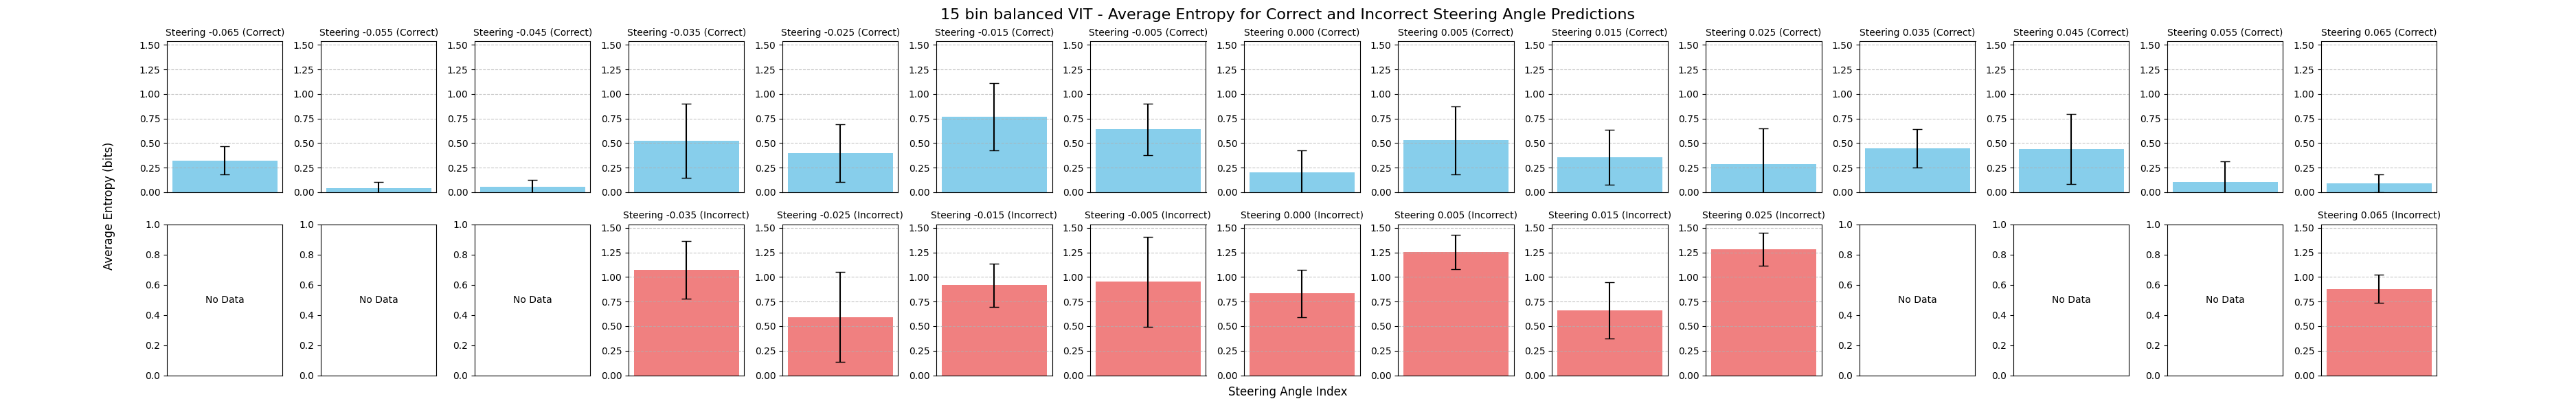
\includegraphics[width=1\linewidth]{Figures/Results/15_bins_vit_entropy_plot_balanced.png}
%     \caption{Average Entropy for Correct and Incorrect Steering Angles Predictions for the 15-Bin vit Model on a balanced Dataset, with Error Bars Indicating Standard Deviation.}
%     \label{fig:15_bins_vit_entropy_balanced}
% \end{figure}
% % 15_BINS_VIT_SOFTMAX_DIST_UNBALANCED

% \subsection{Average Entropy Prediction of vit model trained on 15 bin unbalanced Dataset}

% \begin{figure}[H]
%     \centering
%     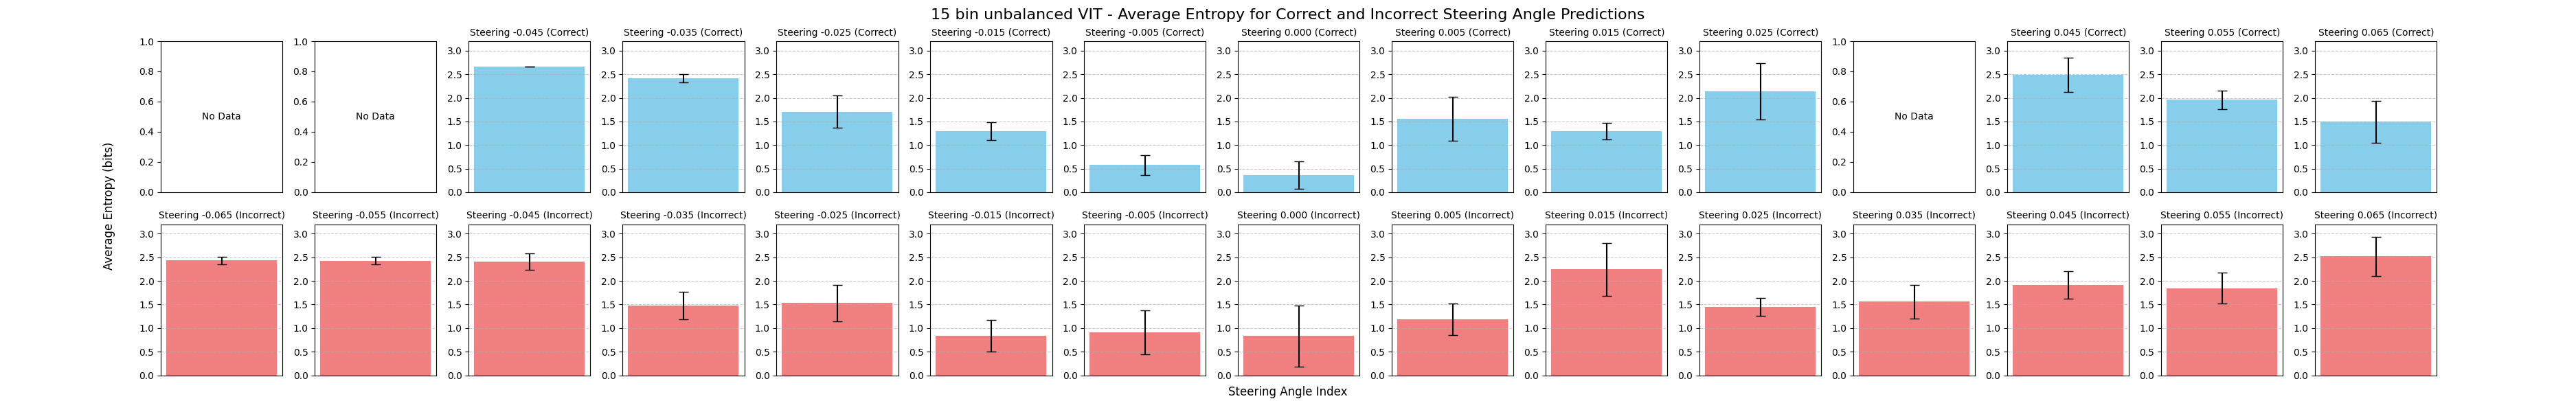
\includegraphics[width=1\linewidth]{Figures/Results/15_bins_vit_entropy_plot_unbalanced.png}
%     \caption{Average Entropy for Correct and Incorrect Steering Angles Predictions for the 15-Bin vit Model on a unbalanced Dataset, with Error Bars Indicating Standard Deviation.}
%     \label{fig:15_bins_vit_entropy_unbalanced}
% \end{figure}
% % 3_BINS_CNN_SOFTMAX_DIST_BALANCED

% \subsection{Average Entropy Prediction of cnn model trained on 3 bin balanced Dataset}

% \begin{figure}[H]
%     \centering
%     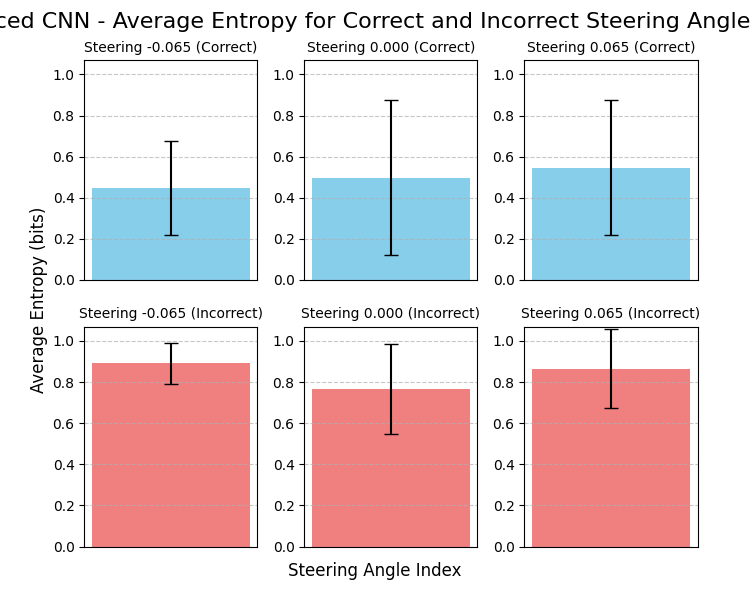
\includegraphics[width=1\linewidth]{Figures/Results/3_bins_cnn_entropy_plot_balanced.png}
%     \caption{Average Entropy for Correct and Incorrect Steering Angles Predictions for the 3-Bin cnn Model on a balanced Dataset, with Error Bars Indicating Standard Deviation.}
%     \label{fig:3_bins_cnn_entropy_balanced}
% \end{figure}
% % 3_BINS_CNN_SOFTMAX_DIST_UNBALANCED

% \subsection{Average Entropy Prediction of cnn model trained on 3 bin unbalanced Dataset}

% \begin{figure}[H]
%     \centering
%     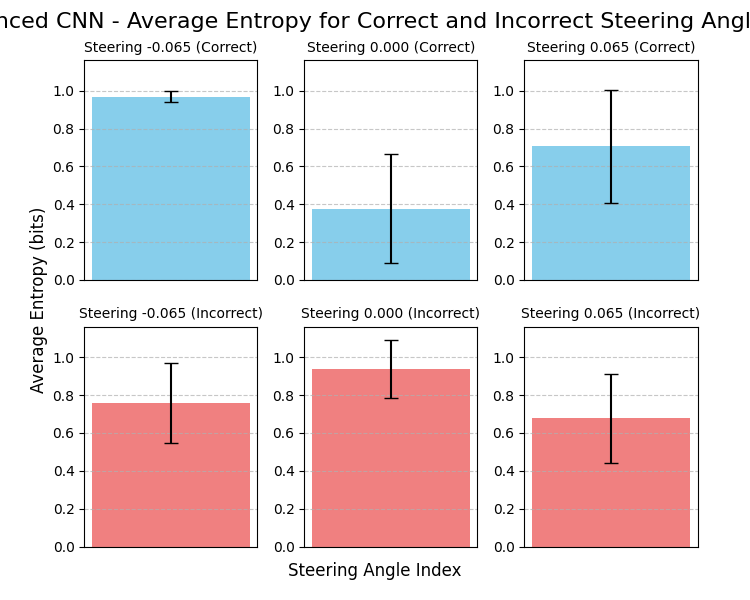
\includegraphics[width=1\linewidth]{Figures/Results/3_bins_cnn_entropy_plot_unbalanced.png}
%     \caption{Average Entropy for Correct and Incorrect Steering Angles Predictions for the 3-Bin cnn Model on a unbalanced Dataset, with Error Bars Indicating Standard Deviation.}
%     \label{fig:3_bins_cnn_entropy_unbalanced}
% \end{figure}
% % 3_BINS_VIT_SOFTMAX_DIST_BALANCED

% \subsection{Average Entropy Prediction of vit model trained on 3 bin balanced Dataset}

% \begin{figure}[H]
%     \centering
%     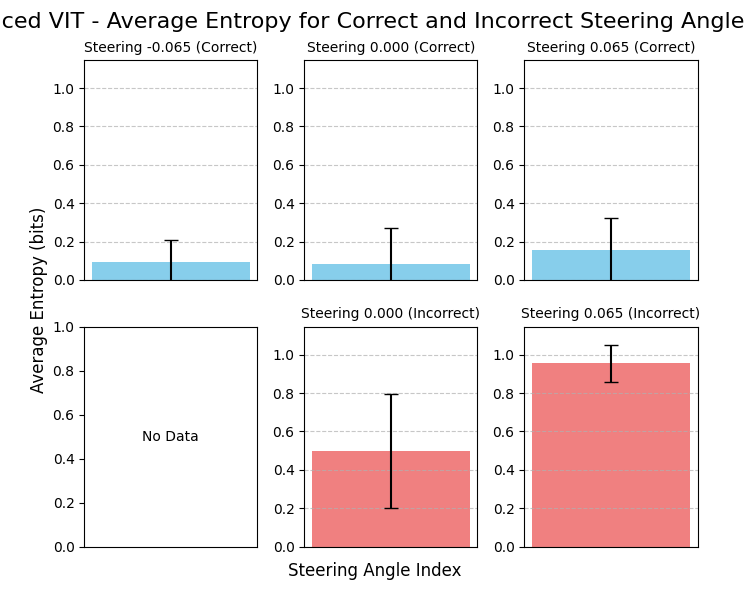
\includegraphics[width=1\linewidth]{Figures/Results/3_bins_vit_entropy_plot_balanced.png}
%     \caption{Average Entropy for Correct and Incorrect Steering Angles Predictions for the 3-Bin vit Model on a balanced Dataset, with Error Bars Indicating Standard Deviation.}
%     \label{fig:3_bins_vit_entropy_balanced}
% \end{figure}
% % 3_BINS_VIT_SOFTMAX_DIST_UNBALANCED

% \subsection{Average Entropy Prediction of vit model trained on 3 bin unbalanced Dataset}

% \begin{figure}[H]
%     \centering
%     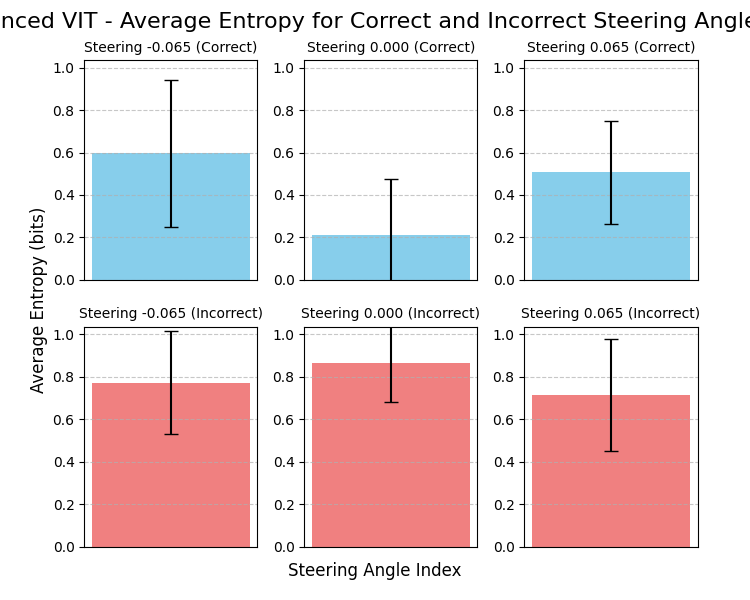
\includegraphics[width=1\linewidth]{Figures/Results/3_bins_vit_entropy_plot_unbalanced.png}
%     \caption{Average Entropy for Correct and Incorrect Steering Angles Predictions for the 3-Bin vit Model on a unbalanced Dataset, with Error Bars Indicating Standard Deviation.}
%     \label{fig:3_bins_vit_entropy_unbalanced}
% \end{figure}
% % 5_BINS_CNN_SOFTMAX_DIST_BALANCED

% \subsection{Average Entropy Prediction of cnn model trained on 5 bin balanced Dataset}

% \begin{figure}[H]
%     \centering
%     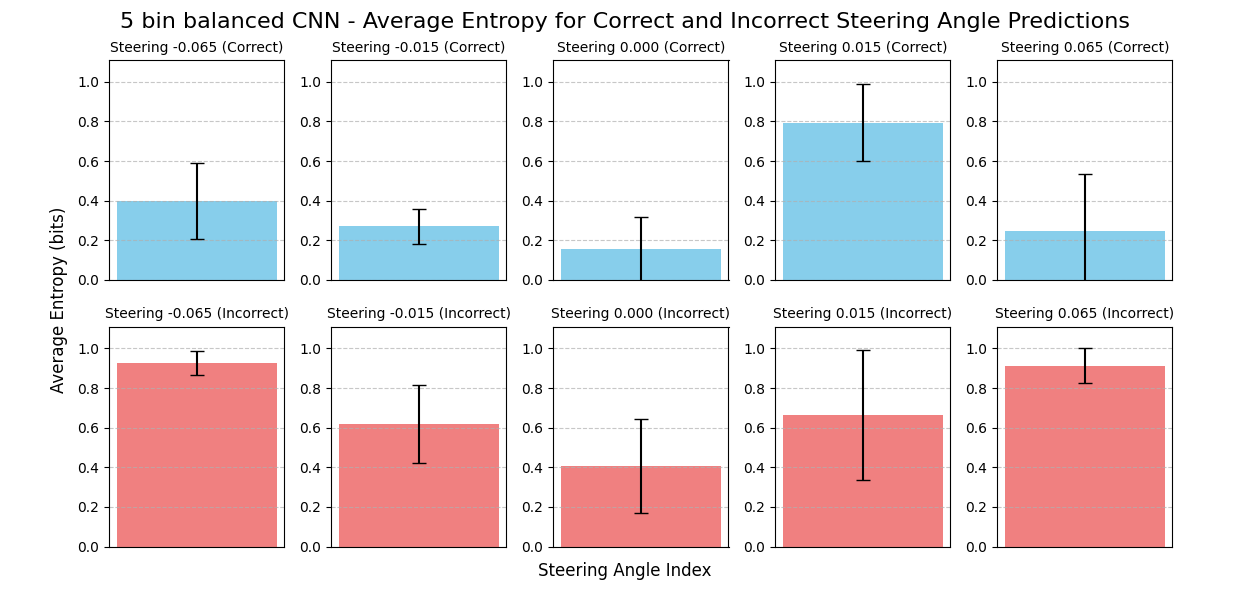
\includegraphics[width=1\linewidth]{Figures/Results/5_bins_cnn_entropy_plot_balanced.png}
%     \caption{Average Entropy for Correct and Incorrect Steering Angles Predictions for the 5-Bin cnn Model on a balanced Dataset, with Error Bars Indicating Standard Deviation.}
%     \label{fig:5_bins_cnn_entropy_balanced}
% \end{figure}
% % 5_BINS_CNN_SOFTMAX_DIST_UNBALANCED

% \subsection{Average Entropy Prediction of cnn model trained on 5 bin unbalanced Dataset}

% \begin{figure}[H]
%     \centering
%     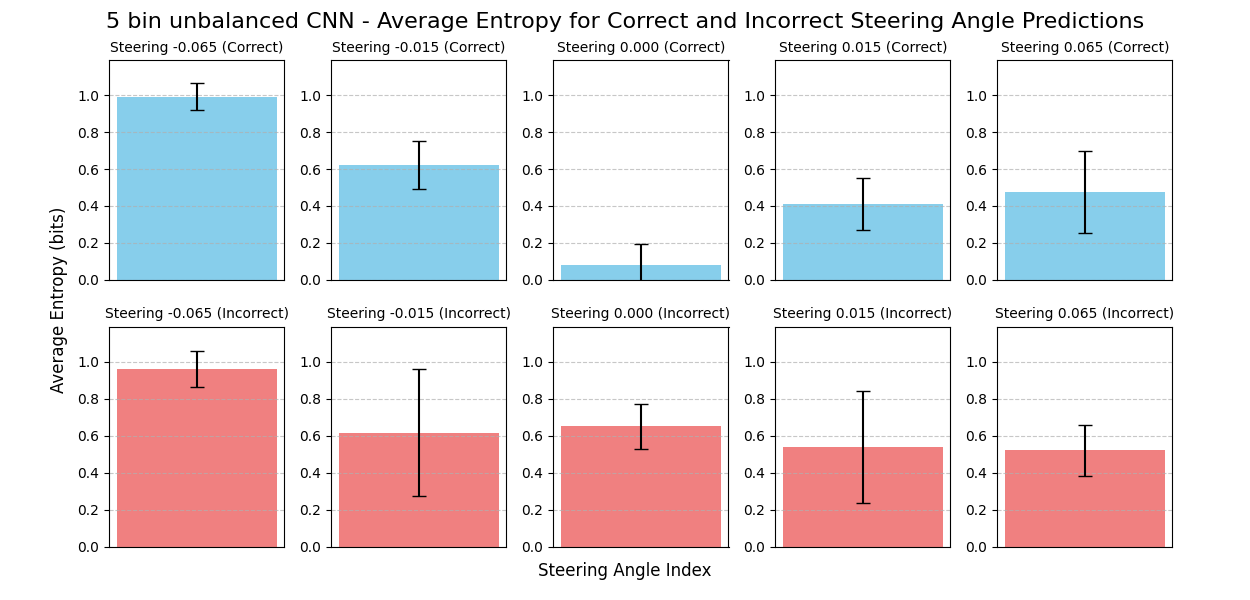
\includegraphics[width=1\linewidth]{Figures/Results/5_bins_cnn_entropy_plot_unbalanced.png}
%     \caption{Average Entropy for Correct and Incorrect Steering Angles Predictions for the 5-Bin cnn Model on a unbalanced Dataset, with Error Bars Indicating Standard Deviation.}
%     \label{fig:5_bins_cnn_entropy_unbalanced}
% \end{figure}
% % 5_BINS_VIT_SOFTMAX_DIST_BALANCED

% \subsection{Average Entropy Prediction of vit model trained on 5 bin balanced Dataset}

% \begin{figure}[H]
%     \centering
%     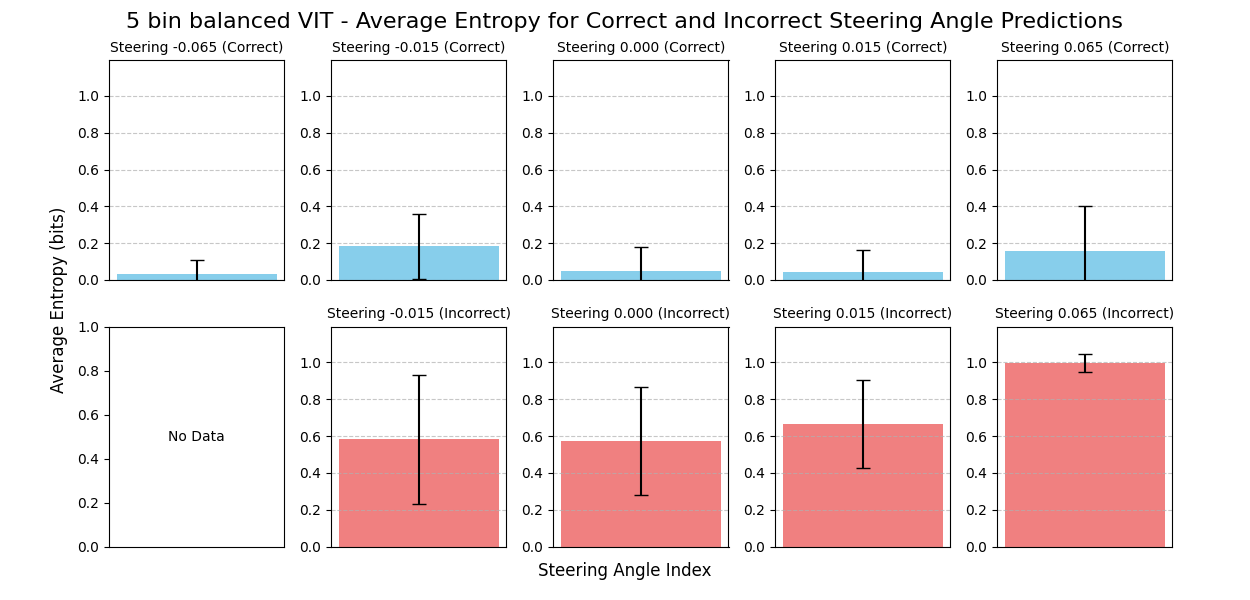
\includegraphics[width=1\linewidth]{Figures/Results/5_bins_vit_entropy_plot_balanced.png}
%     \caption{Average Entropy for Correct and Incorrect Steering Angles Predictions for the 5-Bin vit Model on a balanced Dataset, with Error Bars Indicating Standard Deviation.}
%     \label{fig:5_bins_vit_entropy_balanced}
% \end{figure}
% % 5_BINS_VIT_SOFTMAX_DIST_UNBALANCED

% \subsection{Average Entropy Prediction of vit model trained on 5 bin unbalanced Dataset}

% \begin{figure}[H]
%     \centering
%     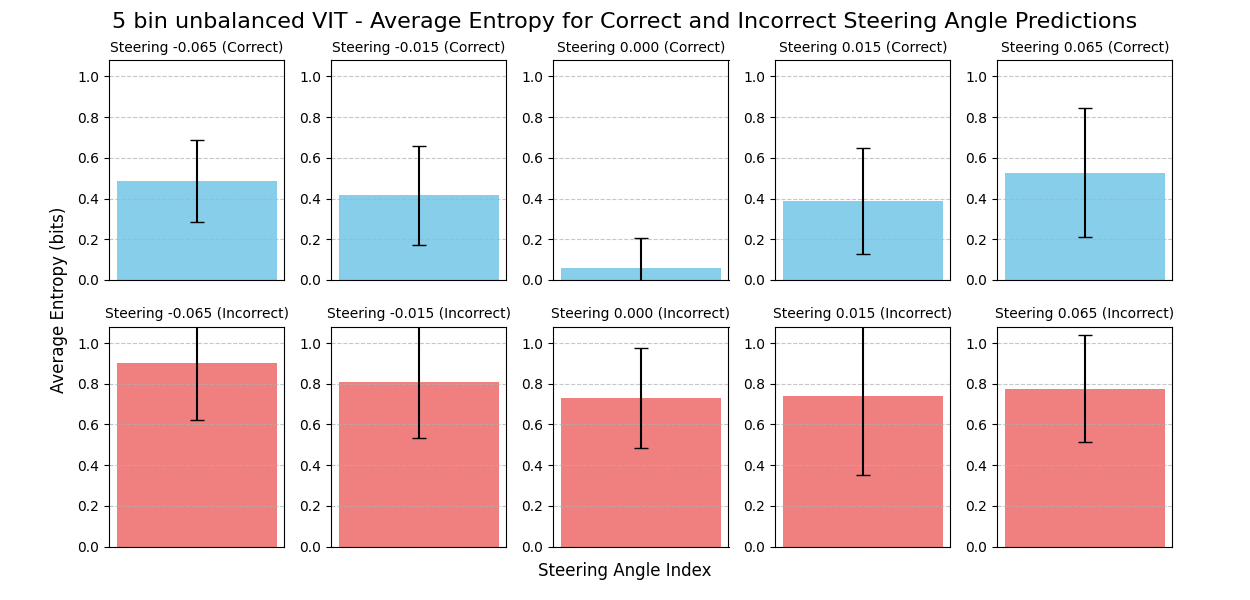
\includegraphics[width=1\linewidth]{Figures/Results/5_bins_vit_entropy_plot_unbalanced.png}
%     \caption{Average Entropy for Correct and Incorrect Steering Angles Predictions for the 5-Bin vit Model on a unbalanced Dataset, with Error Bars Indicating Standard Deviation.}
%     \label{fig:5_bins_vit_entropy_unbalanced}
% \end{figure}
% \begin{enumerate}
%     \item For self-driving softmax analysis, threshold based on class
%     \item Different types of noise
%     \item Similarity Indexes
%     \item ViT 5 bin needs more experiments at lower noise levels, such as the ViT 3 bin model was subject to (1, 2, 3, 4, 5, 6 and 7\%) to determine if both are equally sensitive to noise.
%     \item Fiducial markers, in addition to 
% \end{enumerate}

% While the RegCNNCUFid (Table \ref{results:table_regression_models}) model showed a lower D MAE (0.0461) compared to RegCNNCU (0.0588), this difference may be attributable to statistical noise rather than a robust effect. Nonetheless, the use of fiducial markers remains a promising direction and warrants further investigation with controlled experiments.

% Overall Accuracy for CNN classifiers is consistently higher for models trained on unbalanced datasets, while the trend is inverted for ViT classifiers. This may be related to dataset sizes and network capacity. The hypothesis is that the CNN being a relative small model with in the order of 200k trainable parameters, learned the smaller, unbalanced datasets better, while the ViT architecture used for comparison has in the order of 85M trainable parameters, learned the larger datasets better. Dataset size could be used a a training hyperparameter in determining if there is an optimal data quantity the model could learn, correlating to number of trainable parameters, that is approaching the problem from the dataset size and calibration to adjust to the number of parameters, instead of the traditional approach, of changing model size and ultimately number of parameters to learn a dataset.